\documentclass{article}

% content/resources/templates/preamble.tex
\usepackage[margin=0.6in]{geometry}
\author{Milav Dabgar}
\usepackage{amsmath,amssymb,amsthm}
\usepackage{booktabs}
\usepackage{multirow}
\usepackage{xcolor}
\usepackage{tcolorbox}
\tcbuselibrary{breakable,skins}
\usepackage[colorlinks=true,linkcolor=blue]{hyperref}
\usepackage{titlesec}
\usepackage{enumitem}
\usepackage{tikz}
\usepackage{pgfplots}
\usepackage{circuitikz}
\usepackage[version=4]{mhchem}
\usepackage{longtable}
\usepackage{array}
\usepackage{float}
\usepackage{caption}
\usepackage{listings}

\lstset{
  basicstyle=\small\ttfamily,
  breaklines=true,
  breakatwhitespace=false,
  postbreak=\mbox{\textcolor{red}{$\hookrightarrow$}\space},
  float=false,
  numbers=left,
  numberstyle=\tiny\color{gray},
  numbersep=10pt,
  xleftmargin=2em,
  keywordstyle=\color{blue},
  commentstyle=\color{green!60!black},
  stringstyle=\color{purple},
  backgroundcolor=\color{gray!5},
  showstringspaces=false,
  tabsize=2,
  captionpos=b,
  keepspaces=true,
  columns=flexible
}

\pgfplotsset{compat=1.18}
\usetikzlibrary{shapes,arrows,positioning,calc,patterns,decorations.pathmorphing,decorations.markings,arrows.meta}

% Color scheme
\definecolor{headcolor}{RGB}{0,102,204}
\definecolor{keycolor}{RGB}{220,20,60}
\definecolor{solutioncolor}{RGB}{34,139,34}
\definecolor{mnemoniccolor}{RGB}{148,0,211}
\definecolor{codecolor}{RGB}{0,0,100}

% Spacing
\setlength{\parskip}{3pt}
\setlist[itemize]{nosep}
\setlist[enumerate]{nosep}

% Title formatting
\titleformat{\section}{\Large\bfseries\color{headcolor}}{\thesection}{1em}{}
\titleformat{\subsection}{\large\bfseries\color{headcolor}}{\thesubsection}{1em}{}

% Pandoc tightlist compatibility
\providecommand{\tightlist}{%
  \setlength{\itemsep}{0pt}\setlength{\parskip}{0pt}}

% Pandoc longtable compatibility
\newcounter{none}
\def\thenone{}


% content/resources/templates/english-boxes.tex
% This file is currently empty - it exists to maintain consistency with the import structure.
% Add custom environments here if needed in the future.


% Custom commands for GTU solutions
% This file defines semantic commands for consistent formatting

% Question command with automatic formatting
\newcommand{\question}[2]{%
  \section*{Question #1}%
  \textbf{#2}%
}

% OR question variant
\newcommand{\questionor}[2]{%
  \section*{Question #1 OR}%
  \textbf{#2}%
}

% Proper table environment with caption
\newenvironment{answertable}[1]{%
  \begin{table}[htbp]
  \centering
  \caption{#1}
}{%
  \end{table}
}

% Proper figure environment for diagrams
\newenvironment{answerdiagram}[1]{%
  \begin{figure}[htbp]
  \centering
  \caption{#1}
}{%
  \end{figure}
}

% Semantic markup for key terms
\newcommand{\keyword}[1]{\textbf{#1}}
\newcommand{\code}[1]{\texttt{#1}}
\newcommand{\classname}[1]{\texttt{#1}}
\newcommand{\methodname}[1]{\texttt{#1}}

% Proper quotation marks
\newcommand{\mnemonic}[1]{``#1''}


\title{Fundamentals of Electrical Engineering (4311101) - Summer 2023 Solution}
\date{August 08, 2023}

\begin{document}
\maketitle

\questionmarks{1(a)}{3}{Define the following term (1) Resistance (2) Electrical energy (3) Electrical Power}

\begin{solutionbox}
\textbf{Answer}:

\begin{center}
\captionof{table}{Definitions of Electrical Terms}
\begin{tabulary}{\linewidth}{|L|L|}
\hline
\textbf{Term} & \textbf{Definition} \\ \hline
\textbf{Resistance} & The property of a material that opposes the flow of electric current, measured in ohms ($\Omega$) \\ \hline
\textbf{Electrical Energy} & The ability to do work by electrical means, measured in joules (J) or kilowatt-hours (kWh) \\ \hline
\textbf{Electrical Power} & The rate at which electrical energy is transferred or converted, measured in watts (W) \\ \hline
\end{tabulary}
\end{center}
\end{solutionbox}

\begin{mnemonicbox}
\mnemonic{RIP: Resistance Impedes Path, Energy Is Potential, Power Is Performance}
\end{mnemonicbox}

\questionmarks{1(b)}{4}{State and Explain Ohm's Law \& write limitations of it.}

\begin{solutionbox}
\textbf{Answer}:

\keyword{Ohm's Law}: The current flowing through a conductor is directly proportional to the voltage across the conductor and inversely proportional to its resistance.

Mathematically: $V = IR$, where:
\begin{itemize}
    \item $V$ = Voltage (volts)
    \item $I$ = Current (amperes)
    \item $R$ = Resistance (ohms)
\end{itemize}

\begin{answerdiagram}{Ohm's Law Flowchart}
\begin{tikzpicture}[node distance=2cm, auto]
    \node [gtu input] (V) {Voltage ($V$)};
    \node [gtu process, right=1.5cm of V] (I) {Current ($I$)};
    \node [gtu block, below=1cm of I] (R) {Resistance ($R$)};

    \path [gtu arrow] (V) -- (I);
    \path [gtu arrow] (R) -- node[left] {Limits} (I);
\end{tikzpicture}
\end{answerdiagram}

\keyword{Limitations of Ohm's Law}:
\begin{itemize}
    \item Not applicable to non-linear devices (semiconductors, gas discharge tubes)
    \item Doesn't hold at high temperatures
    \item Not valid for unilateral elements (diodes)
    \item Fails for time-varying currents
\end{itemize}
\end{solutionbox}

\begin{mnemonicbox}
\mnemonic{VIRO: Voltage Is Resistance times Output current}
\end{mnemonicbox}

\questionmarks{1(c)}{7}{Explain series and parallel connection of batteries.}

\begin{solutionbox}
\textbf{Answer}:

\keyword{Series Connection of Batteries:}

\begin{answerdiagram}{Series Batteries Connection}
\begin{circuitikz}[american voltages]
    \draw (0,0) to[battery1, l=$B_1$] (2,0)
          to[battery1, l=$B_2$] (4,0)
          to[battery1, l=$B_3$] (6,0)
          to[short] (6,-2)
          to[R, l=Load] (0,-2)
          to[short] (0,0);
\end{circuitikz}
\end{answerdiagram}

\keyword{Characteristics of Series Connection:}
\begin{itemize}
    \item \keyword{Total Voltage} = Sum of individual voltages ($V = V_1 + V_2 + ... + V_n$)
    \item \keyword{Current} = Same through all batteries
    \item \keyword{Applications}: Higher voltage requirements
    \item \keyword{Internal Resistance}: Increases ($R_s = r_1 + r_2 + ... + r_n$)
\end{itemize}

\keyword{Parallel Connection of Batteries:}

\begin{answerdiagram}{Parallel Batteries Connection}
\begin{circuitikz}[american voltages]
    \draw (0,2) to[battery1, l=$B_1$] (4,2);
    \draw (0,1) to[battery1, l=$B_2$] (4,1);
    \draw (0,0) to[battery1, l=$B_3$] (4,0);
    
    \draw (0,2) -- (0,0);
    \draw (4,2) -- (4,0);
    
    \draw (0,0) -- (0,-2) -- (1,-2);
    \draw (4,0) -- (4,-2) -- (3,-2);
    \draw (1,-2) to[R, l=Load] (3,-2);
\end{circuitikz}
\end{answerdiagram}

\keyword{Characteristics of Parallel Connection:}
\begin{itemize}
    \item \keyword{Voltage} = Same as individual battery (if identical)
    \item \keyword{Total Current} = Sum of individual currents ($I = I_1 + I_2 + ... + I_n$)
    \item \keyword{Applications}: Higher current capacity required
    \item \keyword{Internal Resistance}: Decreases ($1/R_p = 1/r_1 + 1/r_2 + ... + 1/r_n$)
\end{itemize}
\end{solutionbox}

\begin{mnemonicbox}
\mnemonic{VSCP: Voltage Sums in Series, Current Parallels}
\end{mnemonicbox}

\questionmarks{1(c) OR}{7}{Explain series and parallel connection of Resistors.}

\begin{solutionbox}
\textbf{Answer}:

\keyword{Series Connection of Resistors:}

\begin{answerdiagram}{Series Resistors Connection}
\begin{circuitikz}[american resistors]
    \draw (0,0) to[V, l=Source] (0,2)
          to[R, l=$R_1$] (2,2)
          to[R, l=$R_2$] (4,2)
          to[R, l=$R_3$] (6,2)
          to[short] (6,0)
          to[short] (0,0);
\end{circuitikz}
\end{answerdiagram}

\keyword{Characteristics of Series Connection:}
\begin{itemize}
    \item \keyword{Equivalent Resistance} = Sum of individual resistances ($R_s = R_1 + R_2 + ... + R_n$)
    \item \keyword{Current} = Same through all resistors
    \item \keyword{Voltage} = Divided across resistors proportional to resistance values
    \item \keyword{Power} divided as per voltage distribution
\end{itemize}

\keyword{Parallel Connection of Resistors:}

\begin{answerdiagram}{Parallel Resistors Connection}
\begin{circuitikz}[american resistors]
    \draw (0,0) to[V, l=Source] (0,3);
    \draw (0,3) -- (6,3);
    
    \draw (2,3) to[R, l=$R_1$] (2,0);
    \draw (4,3) to[R, l=$R_2$] (4,0);
    \draw (6,3) to[R, l=$R_3$] (6,0);
    
    \draw (0,0) -- (6,0);
\end{circuitikz}
\end{answerdiagram}

\keyword{Characteristics of Parallel Connection:}
\begin{itemize}
    \item \keyword{Equivalent Resistance}: $1/R_p = 1/R_1 + 1/R_2 + ... + 1/R_n$
    \item \keyword{Voltage} = Same across all resistors
    \item \keyword{Current} = Divided inverse-proportionally to resistance values
    \item \keyword{Total Current} = Sum of individual currents
\end{itemize}
\end{solutionbox}

\begin{mnemonicbox}
\mnemonic{RISE-VICE: Resistance Increases in Series, Voltage Is Constant in Every parallel}
\end{mnemonicbox}

\questionmarks{2(a)}{3}{Define: (1) Amplitude (2) Frequency (3) Time period}

\begin{solutionbox}
\textbf{Answer}:

\begin{center}
\captionof{table}{Definitions of Waveform Terms}
\begin{tabulary}{\linewidth}{|L|L|}
\hline
\textbf{Term} & \textbf{Definition} \\ \hline
\textbf{Amplitude} & Maximum displacement of a waveform from its mean position, measured in volts or amperes \\ \hline
\textbf{Frequency} & Number of complete cycles occurring in one second, measured in hertz (Hz) \\ \hline
\textbf{Time Period} & Time taken to complete one cycle of waveform, measured in seconds (s) \\ \hline
\end{tabulary}
\end{center}
\end{solutionbox}

\begin{mnemonicbox}
\mnemonic{AFT: Amplitude is the Full height, Time period is the Total cycle}
\end{mnemonicbox}

\questionmarks{2(b)}{4}{10$\Omega$, 20$\Omega$ and 30$\Omega$ resistors are connected in series and 100V supply is given to them. Find (1) Equivalent resistance (2) Circuit current (3) Voltage drop across each Resistor (4) Power loss in each resistor.}

\begin{solutionbox}
\textbf{Answer}:

\begin{answerdiagram}{Series Circuit Problem}
\begin{circuitikz}[american resistors]
    \draw (0,0) to[V, l=100V] (0,2)
          to[R, l=10$\Omega$] (2,2)
          to[R, l=20$\Omega$] (4,2)
          to[R, l=30$\Omega$] (6,2)
          to[short] (6,0)
          to[short] (0,0);
\end{circuitikz}
\end{answerdiagram}

\keyword{Solution:}

\begin{center}
\captionof{table}{Calculations}
\begin{tabulary}{\linewidth}{|L|L|L|}
\hline
\textbf{Parameter} & \textbf{Calculation} & \textbf{Result} \\ \hline
Equivalent Resistance & $R = 10\Omega + 20\Omega + 30\Omega$ & $60\Omega$ \\ \hline
Circuit Current & $I = 100\text{V}/60\Omega$ & $1.67\text{A}$ \\ \hline
Voltage across 10$\Omega$ & $V_1 = 1.67\text{A} \times 10\Omega$ & $16.7\text{V}$ \\ \hline
Voltage across 20$\Omega$ & $V_2 = 1.67\text{A} \times 20\Omega$ & $33.3\text{V}$ \\ \hline
Voltage across 30$\Omega$ & $V_3 = 1.67\text{A} \times 30\Omega$ & $50.0\text{V}$ \\ \hline
Power in 10$\Omega$ & $P_1 = 1.67^2 \times 10$ & $27.8\text{W}$ \\ \hline
Power in 20$\Omega$ & $P_2 = 1.67^2 \times 20$ & $55.6\text{W}$ \\ \hline
Power in 30$\Omega$ & $P_3 = 1.67^2 \times 30$ & $83.4\text{W}$ \\ \hline
\end{tabulary}
\end{center}
\end{solutionbox}

\begin{mnemonicbox}
\mnemonic{RE\c{C}VP: Resistances Equivalent Causes Voltage and Power division}
\end{mnemonicbox}

\questionmarks{2(c)}{7}{Explain A.C Through pure Resistor with wave form \& vector diagram.}

\begin{solutionbox}
\textbf{Answer}:

In a pure resistive circuit with AC supply:

\keyword{Key Characteristics:}
\begin{itemize}
    \item Current and voltage are \keyword{in phase} with each other
    \item Circuit follows Ohm's Law: $V = IR$
    \item Power is always positive ($P = VI$)
    \item No reactive power consumed
    \item Power factor = 1 ($\cos \phi = 1$)
\end{itemize}

\begin{answerdiagram}{Waveform and Vector Diagram for Pure Resistor}
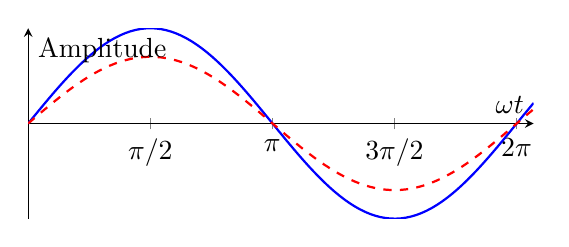
\begin{tikzpicture}
    % Waveform
    \begin{axis}[
        width=8cm, height=4cm,
        axis lines=middle,
        xlabel=$\omega t$, ylabel=Amplitude,
        xtick={0, 1.57, 3.14, 4.71, 6.28},
        xticklabels={0, $\pi/2$, $\pi$, $3\pi/2$, $2\pi$},
        ytick=\empty,
        domain=0:6.5, samples=100
    ]
        \addplot[blue, thick] {sin(deg(x))} node[right] {V};
        \addplot[red, dashed, thick] {0.7*sin(deg(x))} node[right] {I};
    \end{axis}
\end{tikzpicture}
\quad
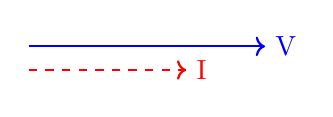
\begin{tikzpicture}
    % Vector Diagram
    \draw[->, thick, blue] (0,0) -- (3,0) node[right] {V};
    \draw[->, thick, red, dashed] (0,-0.3) -- (2,-0.3) node[right] {I};
\end{tikzpicture}
\end{answerdiagram}

\keyword{Vector Diagram Notes:} Matches phase (Parallel vectors).
\end{solutionbox}

\begin{mnemonicbox}
\mnemonic{PARVIP: Pure AC Resistor has Voltage In Phase with current}
\end{mnemonicbox}

\questionmarks{2(a) OR}{3}{Define: (1) cycle (2) Form factor (3) Peak factor}

\begin{solutionbox}
\textbf{Answer}:

\begin{center}
\captionof{table}{AC Term Definitions}
\begin{tabulary}{\linewidth}{|L|L|}
\hline
\textbf{Term} & \textbf{Definition} \\ \hline
\textbf{Cycle} & One complete repetition of a periodic waveform from start point to same point again \\ \hline
\textbf{Form Factor} & Ratio of RMS value to average value of AC waveform (For sine wave = 1.11) \\ \hline
\textbf{Peak Factor} & Ratio of maximum value to RMS value of AC waveform (For sine wave = 1.414) \\ \hline
\end{tabulary}
\end{center}
\end{solutionbox}

\begin{mnemonicbox}
\mnemonic{CFP: Cycle Finishes a Pattern, Form Factor = Vrms/Vavg, Peak Factor = Vmax/Vrms}
\end{mnemonicbox}

\questionmarks{2(b) OR}{4}{20$\Omega$, 30$\Omega$ and 50$\Omega$ resistors are connected in parallel and 60V supply is given to them. Find (1) Current in each Resistor. (2) Total current (3) Equivalent resistance (4) Power loss in each resistor.}

\begin{solutionbox}
\textbf{Answer}:

\begin{answerdiagram}{Parallel Circuit Problem}
\begin{circuitikz}[american resistors]
    \draw (0,0) to[V, l=60V] (0,3);
    \draw (0,3) -- (6,3);
    \draw (2,3) to[R, l=20$\Omega$] (2,0);
    \draw (4,3) to[R, l=30$\Omega$] (4,0);
    \draw (6,3) to[R, l=50$\Omega$] (6,0);
    \draw (0,0) -- (6,0);
\end{circuitikz}
\end{answerdiagram}

\keyword{Solution:}

\begin{center}
\captionof{table}{Calculations}
\begin{tabulary}{\linewidth}{|L|L|L|}
\hline
\textbf{Parameter} & \textbf{Calculation} & \textbf{Result} \\ \hline
Current in 20$\Omega$ & $I_1 = 60\text{V}/20\Omega$ & $3\text{A}$ \\ \hline
Current in 30$\Omega$ & $I_2 = 60\text{V}/30\Omega$ & $2\text{A}$ \\ \hline
Current in 50$\Omega$ & $I_3 = 60\text{V}/50\Omega$ & $1.2\text{A}$ \\ \hline
Total Current & $I = 3\text{A} + 2\text{A} + 1.2\text{A}$ & $6.2\text{A}$ \\ \hline
Equivalent Resistance & $1/R_{eq} = 1/20 + 1/30 + 1/50$ & $9.68\Omega$ \\ \hline
Power in 20$\Omega$ & $P_1 = 60\text{V} \times 3\text{A}$ & $180\text{W}$ \\ \hline
Power in 30$\Omega$ & $P_2 = 60\text{V} \times 2\text{A}$ & $120\text{W}$ \\ \hline
Power in 50$\Omega$ & $P_3 = 60\text{V} \times 1.2\text{A}$ & $72\text{W}$ \\ \hline
\end{tabulary}
\end{center}
\end{solutionbox}

\begin{mnemonicbox}
\mnemonic{VICTIM: Voltage Is Constant, Total current Is the Measure (in parallel)}
\end{mnemonicbox}

\questionmarks{2(c) OR}{7}{Explain A.C Through pure capacitor with wave form \& vector diagram.}

\begin{solutionbox}
\textbf{Answer}:

In a pure capacitive circuit with AC supply:

\keyword{Key Characteristics:}
\begin{itemize}
    \item Current \keyword{leads} voltage by $90^\circ$ 
    \item Capacitive reactance $X_c = 1/(2\pi fC)$
    \item Only reactive power (no active power)
    \item Power factor = 0 (lagging)
    \item Average power over complete cycle = 0
\end{itemize}

\begin{answerdiagram}{Waveform and Vector Diagram for Pure Capacitor}
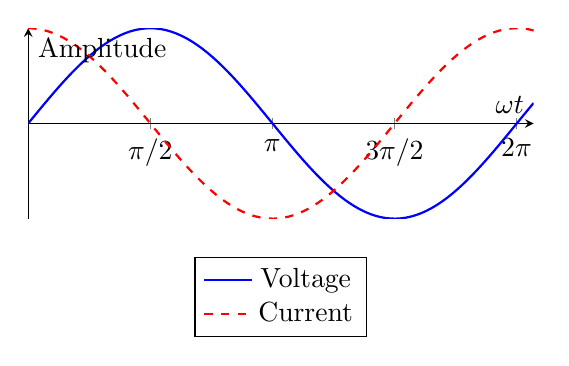
\begin{tikzpicture}
    % Waveform
    \begin{axis}[
        width=8cm, height=4cm,
        axis lines=middle,
        xlabel=$\omega t$, ylabel=Amplitude,
        xtick={0, 1.57, 3.14, 4.71, 6.28},
        xticklabels={0, $\pi/2$, $\pi$, $3\pi/2$, $2\pi$},
        ytick=\empty,
        domain=0:6.5, samples=100,
        legend style={at={(0.5,-0.2)},anchor=north}
    ]
        \addplot[blue, thick] {sin(deg(x))} node[above] {};
        \addlegendentry{Voltage}
        \addplot[red, dashed, thick] {sin(deg(x)+90)} node[above] {};
        \addlegendentry{Current}
    \end{axis}
\end{tikzpicture}
\quad
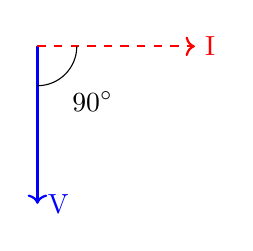
\begin{tikzpicture}
    % Vector Diagram
    \draw[->, thick, blue] (0,0) -- (0,-2) node[right] {V};
    \draw[->, thick, red, dashed] (0,0) -- (2,0) node[right] {I};
    % Draw angle
    \draw[thin] (0.5,0) arc (0:-90:0.5);
    \node at (0.7,-0.7) {$90^\circ$};
\end{tikzpicture}
\end{answerdiagram}

\keyword{Note}: V lags I by $90^\circ$.
\end{solutionbox}

\begin{mnemonicbox}
\mnemonic{CLEAR-90: Capacitive Load has Electrical Angle Reaching 90 degrees (current leads voltage)}
\end{mnemonicbox}

\questionmarks{3(a)}{3}{Define RMS value and average value related to alternating waveform write formula of it.}

\begin{solutionbox}
\textbf{Answer}:

\begin{center}
\captionof{table}{RMS and Average Value Definitions}
\begin{tabulary}{\linewidth}{|L|L|L|}
\hline
\textbf{Term} & \textbf{Definition} & \textbf{Formula} \\ \hline
\textbf{RMS Value} & Root Mean Square value - equivalent DC value producing the same heating effect & $V_{rms} = 0.707 \times V_{max}$ for sine wave \\ \hline
\textbf{Average Value} & Mean value of all instantaneous values over half cycle & $V_{avg} = 0.637 \times V_{max}$ for sine wave \\ \hline
\end{tabulary}
\end{center}
\end{solutionbox}

\begin{mnemonicbox}
\mnemonic{RAM: RMS Averages the Mean square (RMS = 0.707 Vmax, AVG = 0.637 Vmax)}
\end{mnemonicbox}

\questionmarks{3(b)}{4}{If A.C. current is represented by equation $i=25 \sin(314t)$. Calculate (1) R.m.s. value (2) Average value (3) Frequency (4) Time period}

\begin{solutionbox}
\textbf{Answer}:

\textbf{Given equation:} $i = 25 \sin(314t)$

\begin{center}
\captionof{table}{AC Parameter Calculations}
\begin{tabulary}{\linewidth}{|L|L|L|}
\hline
\textbf{Parameter} & \textbf{Calculation} & \textbf{Result} \\ \hline
Maximum value & $I_{max} = 25\text{A}$ & $25\text{A}$ \\ \hline
RMS value & $I_{rms} = I_{max}/\sqrt{2} = 25/1.414$ & $17.68\text{A}$ \\ \hline
Average value & $I_{avg} = 2I_{max}/\pi = 2 \times 25/3.14$ & $15.92\text{A}$ \\ \hline
Angular frequency & $\omega = 314\text{ rad/s}$ & $314\text{ rad/s}$ \\ \hline
Frequency & $f = \omega/2\pi = 314/6.28$ & $50\text{Hz}$ \\ \hline
Time period & $T = 1/f = 1/50$ & $0.02\text{s}$ \\ \hline
\end{tabulary}
\end{center}
\end{solutionbox}

\begin{mnemonicbox}
\mnemonic{SMART: Sine's Maximum divided by root 2 equals RMS Then 2/pi for Average}
\end{mnemonicbox}

\questionmarks{3(c)}{7}{Explain star connection of resistors and Derive equation shows relationship between voltage and current in star connection.}

\begin{solutionbox}
\textbf{Answer}:

\keyword{Star (Y) Connection:}

\begin{answerdiagram}{Star (Y) Connection Diagram}
\begin{circuitikz}
    \draw (0,0) node[anchor=north]{N} to[R, l=$R_1$] (0,2) node[anchor=south]{$L_1$};
    \draw (0,0) to[R, l=$R_2$] (-1.73,-1) node[anchor=north]{$L_2$};
    \draw (0,0) to[R, l=$R_3$] (1.73,-1) node[anchor=north]{$L_3$};
\end{circuitikz}
\end{answerdiagram}

\keyword{Characteristics of Star Connection:}
\begin{itemize}
    \item Three resistors connected at common point (neutral)
    \item Line voltage ($V_L$) = $\sqrt{3} \times$ Phase voltage ($V_{ph}$)
    \item Line current ($I_L$) = Phase current ($I_{ph}$)
    \item For balanced load: $I_L = I_{ph}$
    \item Total power = $3 \times$ Phase power
\end{itemize}

\keyword{Mathematical Relationship:}
\begin{itemize}
    \item Phase voltage: $V_{ph} = V_L/\sqrt{3}$
    \item Phase current: $I_{ph} = I_L$
    \item For balanced resistive load: $I_{ph} = V_{ph}/R$
    \item Therefore: $I_L = V_L/(\sqrt{3} \times R)$
\end{itemize}
\end{solutionbox}

\begin{mnemonicbox}
\mnemonic{SLIP-3: Star Line current Is Phase current, Line voltage is Phase voltage times root-3}
\end{mnemonicbox}

\questionmarks{3(a) OR}{3}{Explain generation of alternating E.M.F.}

\begin{solutionbox}
\textbf{Answer}:

\keyword{Generation of Alternating EMF:}

\begin{answerdiagram}{Rotating Coil in Magnetic Field}
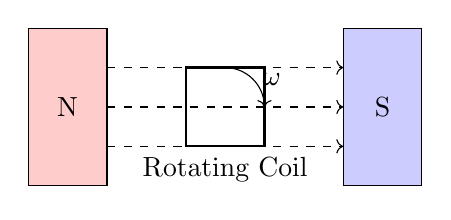
\begin{tikzpicture}
    % Magnets
    \draw[fill=red!20] (-2.5,-1) rectangle (-1.5,1) node[midway]{N};
    \draw[fill=blue!20] (1.5,-1) rectangle (2.5,1) node[midway]{S};
    % Field lines
    \draw[->,dashed] (-1.5,0.5) -- (1.5,0.5);
    \draw[->,dashed] (-1.5,0) -- (1.5,0);
    \draw[->,dashed] (-1.5,-0.5) -- (1.5,-0.5);
    % Coil
    \draw[thick] (-0.5,-0.5) rectangle (0.5,0.5);
    \draw[->] (0,0.5) arc (90:0:0.5) node[midway, right] {$\omega$};
    \node at (0,-0.8) {Rotating Coil};
\end{tikzpicture}
\end{answerdiagram}

\keyword{Process:}
\begin{itemize}
    \item Coil rotates in uniform magnetic field
    \item Flux linkage changes with angle of rotation
    \item Rate of change of flux induces EMF
    \item EMF follows sinusoidal pattern: $e = E_{max} \sin(\omega t)$
    \item Frequency depends on rotation speed
\end{itemize}
\end{solutionbox}

\begin{mnemonicbox}
\mnemonic{FRAME: Flux Rotation Alternates Magnetic EMF}
\end{mnemonicbox}

\questionmarks{3(b) OR}{4}{An alternating EMF is expressed by $e= 100 \sin(2\pi 50t)$. Find out (1) Max value of EMF (2) Frequency (3) Time period (4) Angular Frequency}

\begin{solutionbox}
\textbf{Answer}:

\textbf{Given equation:} $e = 100 \sin(2\pi 50t)$

\begin{center}
\captionof{table}{EMF Parameter Calculations}
\begin{tabulary}{\linewidth}{|L|L|L|}
\hline
\textbf{Parameter} & \textbf{Calculation} & \textbf{Result} \\ \hline
Maximum EMF & $E_{max} = 100\text{V}$ & $100\text{V}$ \\ \hline
Angular Frequency & $\omega = 2\pi 50 = 314\text{ rad/s}$ & $314\text{ rad/s}$ \\ \hline
Frequency & $f = 50\text{Hz}$ (directly from equation) & $50\text{Hz}$ \\ \hline
Time Period & $T = 1/f = 1/50$ & $0.02\text{s}$ \\ \hline
\end{tabulary}
\end{center}
\end{solutionbox}

\begin{mnemonicbox}
\mnemonic{FAST: Frequency And period are reciprocals, Sin's Top value is maximum}
\end{mnemonicbox}

\questionmarks{3(c) OR}{7}{Explain star connection and Derive equation shows relationship between voltage and current in delta connection.}

\begin{solutionbox}
\textbf{Answer}:

\keyword{Delta ($\Delta$) Connection:}

\begin{answerdiagram}{Delta Connection Diagram}
\begin{circuitikz}
    \draw (0,0) to[R, l=$R_3$] (4,0);
    \draw (0,0) to[R, l=$R_1$] (2,3.46);
    \draw (2,3.46) to[R, l=$R_2$] (4,0);
    \node at (0,0) [anchor=east] {$L_1$};
    \node at (2,3.46) [anchor=south] {$L_2$};
    \node at (4,0) [anchor=west] {$L_3$};
\end{circuitikz}
\end{answerdiagram}

\keyword{Characteristics of Delta Connection:}
\begin{itemize}
    \item Three resistors connected in closed loop
    \item Line voltage ($V_L$) = Phase voltage ($V_{ph}$)
    \item Line current ($I_L$) = $\sqrt{3} \times$ Phase current ($I_{ph}$)
    \item For balanced load: $V_{ph} = V_L$
    \item Total power = $3 \times$ Phase power
\end{itemize}

\keyword{Mathematical Relationship:}
\begin{itemize}
    \item Phase voltage: $V_{ph} = V_L$
    \item Phase current: $I_{ph} = V_{ph}/R$
    \item Line current: $I_L = \sqrt{3} \times I_{ph}$
    \item Therefore: $I_L = \sqrt{3} \times V_L/R$
\end{itemize}
\end{solutionbox}

\begin{mnemonicbox}
\mnemonic{DELVIr3: Delta Equal Line Voltage, Its line current equals phase current times root-3}
\end{mnemonicbox}

\questionmarks{4(a)}{3}{Define (1) M.M.F. (2) Reluctance (3) flux}

\begin{solutionbox}
\textbf{Answer}:

\begin{center}
\captionof{table}{Magnetic Terms Definitions}
\begin{tabulary}{\linewidth}{|L|L|}
\hline
\textbf{Term} & \textbf{Definition} \\ \hline
\textbf{M.M.F. (Magnetomotive Force)} & The force that produces magnetic flux in a magnetic circuit, measured in ampere-turns (AT) \\ \hline
\textbf{Reluctance} & The magnetic equivalent of resistance, opposition to magnetic flux, measured in AT/Wb \\ \hline
\textbf{Flux} & The total magnetic field passing through a surface, measured in webers (Wb) \\ \hline
\end{tabulary}
\end{center}
\end{solutionbox}

\begin{mnemonicbox}
\mnemonic{MFR: MMF Flows against Reluctance like current flows against resistance}
\end{mnemonicbox}

\questionmarks{4(b)}{4}{Explain Apparent, Active and Reactive power in A.C circuits.}

\begin{solutionbox}
\textbf{Answer}:

\begin{center}
\captionof{table}{AC Power Types}
\begin{tabulary}{\linewidth}{|L|L|L|}
\hline
\textbf{Power Type} & \textbf{Symbol \& Unit} & \textbf{Definition} \\ \hline
\textbf{Apparent Power} & $S$ (VA) & Vector sum of active and reactive power \\ \hline
\textbf{Active Power} & $P$ (W) & Actual work-producing power consumed by the load \\ \hline
\textbf{Reactive Power} & $Q$ (VAR) & Power that oscillates between source and load \\ \hline
\end{tabulary}
\end{center}

\keyword{Power Triangle:}

\begin{answerdiagram}{Power Triangle}
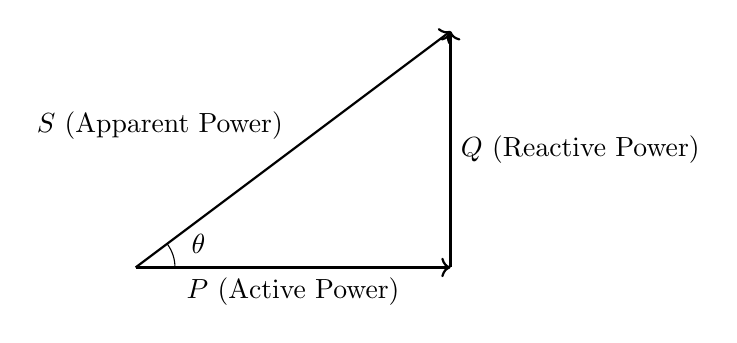
\begin{tikzpicture}
    \draw[->, thick] (0,0) -- (4,0) node[midway, below] {$P$ (Active Power)};
    \draw[->, thick] (4,0) -- (4,3) node[midway, right] {$Q$ (Reactive Power)};
    \draw[->, thick] (0,0) -- (4,3) node[midway, above left] {$S$ (Apparent Power)};
    \draw (0.5,0) arc (0:36.87:0.5);
    \node at (0.8,0.3) {$\theta$};
\end{tikzpicture}
\end{answerdiagram}

\keyword{Relationships:}
\begin{itemize}
    \item $S = \sqrt{P^2 + Q^2}$
    \item $P = S \times \cos \theta$
    \item $Q = S \times \sin \theta$
    \item Power factor = $\cos \theta = P/S$
\end{itemize}
\end{solutionbox}

\begin{mnemonicbox}
\mnemonic{SPARQ: S is Power Apparent, Real is P, Q is reactive}
\end{mnemonicbox}

\questionmarks{4(c)}{7}{Compare electric and magnetic circuit.}

\begin{solutionbox}
\textbf{Answer}:

\begin{center}
\captionof{table}{Electric vs Magnetic Circuit}
\begin{tabulary}{\linewidth}{|L|L|L|}
\hline
\textbf{Parameter} & \textbf{Electric Circuit} & \textbf{Magnetic Circuit} \\ \hline
\textbf{Force} & EMF (V) & MMF (AT) \\ \hline
\textbf{Opposition} & Resistance ($\Omega$) & Reluctance (AT/Wb) \\ \hline
\textbf{Flow} & Current (A) & Flux (Wb) \\ \hline
\textbf{Ohm's Law} & $V = IR$ & MMF = $\Phi \times S$ \\ \hline
\textbf{Medium} & Conductor & Ferromagnetic material \\ \hline
\textbf{Energy} & Stored in electric field & Stored in magnetic field \\ \hline
\textbf{Leakage} & Negligible & Significant \\ \hline
\textbf{Path} & Conductors & Usually closed loop \\ \hline
\textbf{Material Property} & Conductivity & Permeability \\ \hline
\textbf{Current Flow} & Electron flow & No particle flow \\ \hline
\end{tabulary}
\end{center}
\end{solutionbox}

\begin{mnemonicbox}
\mnemonic{VIRO-MSPhiS: Voltage Is to Resistance as MMF is to Reluctance, Our phi flows Similar}
\end{mnemonicbox}

\questionmarks{4(a) OR}{3}{State and explain Fleming's left hand rule.}

\begin{solutionbox}
\textbf{Answer}:

\keyword{Fleming's Left Hand Rule:} Used to find the direction of the force experienced by a current-carrying conductor placed in a magnetic field.

\begin{answerdiagram}{Fleming's Left Hand Rule}
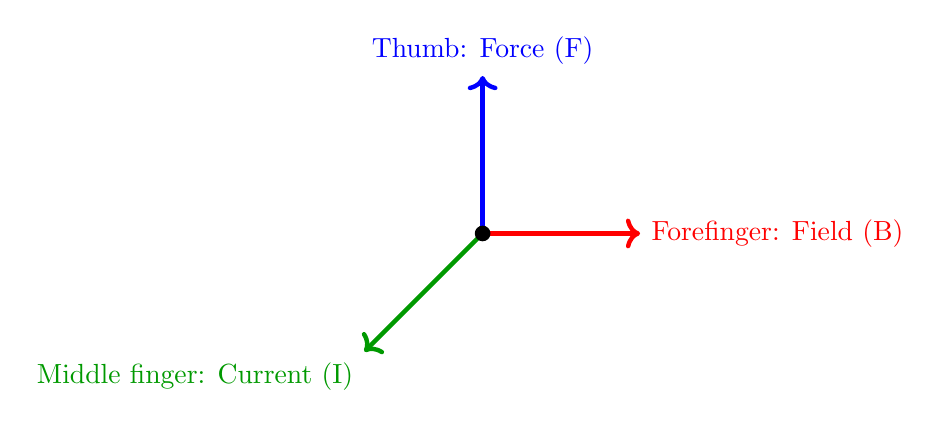
\begin{tikzpicture}
    % Abstract representation
    \draw[->, ultra thick, blue] (0,0) -- (0,2) node[above] {Thumb: Force (F)};
    \draw[->, ultra thick, red] (0,0) -- (2,0) node[right] {Forefinger: Field (B)};
    \draw[->, ultra thick, green!60!black] (0,0) -- (-1.5,-1.5) node[below left] {Middle finger: Current (I)};
    \node at (0,0) [circle, fill=black, inner sep=2pt] {};
\end{tikzpicture}
\end{answerdiagram}

\keyword{Application:}
\begin{itemize}
    \item Thumb $\rightarrow$ Direction of Force (F)
    \item Forefinger $\rightarrow$ Direction of magnetic Field (B)
    \item Middle finger $\rightarrow$ Direction of Current (I)
    \item Only works when fingers are perpendicular to each other
\end{itemize}
\end{solutionbox}

\begin{mnemonicbox}
\mnemonic{FBI-Left: Force, B-field, and I-current directions are shown by the Left hand}
\end{mnemonicbox}

\questionmarks{4(b) OR}{4}{Draw power triangle and explain each component of it.}

\begin{solutionbox}
\textbf{Answer}:

\keyword{Power Triangle:}

\begin{answerdiagram}{Power Triangle Components}
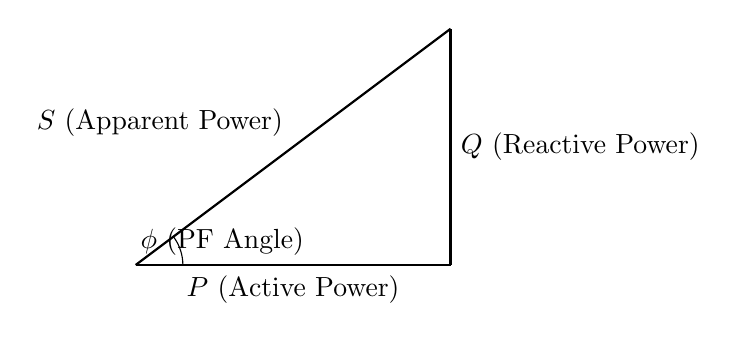
\begin{tikzpicture}
    \draw[thick] (0,0) coordinate (O) -- (4,0) coordinate (P) node[midway, below] {$P$ (Active Power)};
    \draw[thick] (P) -- (4,3) coordinate (Q) node[midway, right] {$Q$ (Reactive Power)};
    \draw[thick] (O) -- (Q) node[midway, above left] {$S$ (Apparent Power)};
    
    \draw (0.6,0) arc (0:36.87:0.6);
    \node at (1.1,0.3) {$\phi$ (PF Angle)};
\end{tikzpicture}
\end{answerdiagram}

\keyword{Components:}
\begin{center}
\captionof{table}{Power Triangle Components}
\begin{tabulary}{\linewidth}{|L|L|L|L|}
\hline
\textbf{Component} & \textbf{Symbol} & \textbf{Unit} & \textbf{Meaning} \\ \hline
\textbf{Active Power} & $P$ & Watt (W) & Real power doing useful work \\ \hline
\textbf{Reactive Power} & $Q$ & VAR & Power oscillating between source and load \\ \hline
\textbf{Apparent Power} & $S$ & VA & Vector sum of $P$ and $Q$ \\ \hline
\textbf{Power Factor} & $\cos \phi$ & - & Ratio of active to apparent power ($P/S$) \\ \hline
\end{tabulary}
\end{center}

\keyword{Relationships:}
\begin{itemize}
    \item $S^2 = P^2 + Q^2$
    \item $P = S \times \cos \phi$
    \item $Q = S \times \sin \phi$
\end{itemize}
\end{solutionbox}

\begin{mnemonicbox}
\mnemonic{SPQR: S is Pythagoras of P and Q, Ratio of P/S is power factor}
\end{mnemonicbox}

\questionmarks{4(c) OR}{7}{Differentiate statically and dynamically induced E.M.F.}

\begin{solutionbox}
\textbf{Answer}:

\begin{center}
\captionof{table}{Statically vs Dynamically Induced EMF}
\begin{tabulary}{\linewidth}{|L|L|L|}
\hline
\textbf{Parameter} & \textbf{Statically Induced EMF} & \textbf{Dynamically Induced EMF} \\ \hline
\textbf{Definition} & EMF induced due to change in current in the primary coil & EMF induced due to relative motion between conductor and magnetic field \\ \hline
\textbf{Mechanism} & Change in linkage flux & Cutting of magnetic flux \\ \hline
\textbf{Movement} & No physical movement required & Requires relative motion \\ \hline
\textbf{Examples} & Transformer, inductor & Generator, motor \\ \hline
\textbf{Faraday's Law} & $e = -N(d\Phi/dt)$ & $e = Blv$ \\ \hline
\textbf{Application} & Power transfer without motion & Power generation through motion \\ \hline
\textbf{Energy Conversion} & Electrical to magnetic and back & Mechanical to electrical or vice versa \\ \hline
\end{tabulary}
\end{center}
\end{solutionbox}

\begin{mnemonicbox}
\mnemonic{STIM-DMOV: STatically Induced needs Magnetic flux change, Dynamically needs MOVement}
\end{mnemonicbox}

\questionmarks{5(a)}{3}{Define (1) solar cell (2) solar panel (3) solar array}

\begin{solutionbox}
\textbf{Answer}:

\begin{center}
\captionof{table}{Solar Term Definitions}
\begin{tabulary}{\linewidth}{|L|L|}
\hline
\textbf{Term} & \textbf{Definition} \\ \hline
\textbf{Solar Cell} & Basic photovoltaic unit that converts sunlight directly into electricity through semiconductor material \\ \hline
\textbf{Solar Panel} & Collection of solar cells connected in series/parallel in a frame \\ \hline
\textbf{Solar Array} & Multiple solar panels connected together to form a larger electricity-generating unit \\ \hline
\end{tabulary}
\end{center}
\end{solutionbox}

\begin{mnemonicbox}
\mnemonic{CPA: Cell Produces electricity, Panel Arrays cells, Array is collection of panels}
\end{mnemonicbox}

\questionmarks{5(b)}{4}{Differentiate HAWT and VAWT.}

\begin{solutionbox}
\textbf{Answer}:

\begin{center}
\captionof{table}{HAWT vs VAWT}
\begin{tabulary}{\linewidth}{|L|L|L|}
\hline
\textbf{Parameter} & \textbf{Horizontal Axis Wind Turbine (HAWT)} & \textbf{Vertical Axis Wind Turbine (VAWT)} \\ \hline
\textbf{Axis Orientation} & Parallel to ground & Perpendicular to ground \\ \hline
\textbf{Efficiency} & Higher (35-45\%) & Lower (15-30\%) \\ \hline
\textbf{Wind Direction} & Needs to face the wind & Works with wind from any direction \\ \hline
\textbf{Generator Location} & At the top of tower & Can be placed at ground level \\ \hline
\textbf{Space Required} & More & Less \\ \hline
\textbf{Noise} & Higher & Lower \\ \hline
\textbf{Examples} & Propeller-type, widely used commercially & Darrieus, Savonius designs \\ \hline
\end{tabulary}
\end{center}
\end{solutionbox}

\begin{mnemonicbox}
\mnemonic{HAVE: Horizontal Aligns with wind, Vertical Enjoys omnidirectional wind}
\end{mnemonicbox}

\questionmarks{5(c)}{7}{Draw and explain the Block diagram of solar power system.}

\begin{solutionbox}
\textbf{Answer}:

\keyword{Solar Power System Block Diagram:}

\begin{answerdiagram}{Solar Power System}
\begin{tikzpicture}[node distance=1.5cm, auto]
    \node [gtu block] (S) {Solar Panel};
    \node [gtu block, right=1cm of S] (C) {Charge\\Controller};
    \node [gtu block, below=1cm of C] (B) {Battery\\Bank};
    \node [gtu block, right=1cm of C] (I) {Inverter};
    \node [gtu block, right=1cm of I] (L) {AC Load};
    \node [gtu block, left=1cm of B] (D) {DC Load};
    
    \path [gtu arrow] (S) -- (C);
    \path [gtu arrow] (C) -- (I);
    \path [gtu arrow] (I) -- (L);
    \path [gtu arrow] (C) edge[bend left] (B);
    \path [gtu arrow] (B) edge[bend left] (C);
    \path [gtu arrow] (B) -- (D);
\end{tikzpicture}
\end{answerdiagram}

\keyword{Components:}
\begin{enumerate}
    \item \keyword{Solar Panels}: Convert sunlight to DC electricity
    \item \keyword{Charge Controller}: Regulates battery charging, prevents overcharging
    \item \keyword{Battery Bank}: Stores energy for use when sunlight isn't available
    \item \keyword{Inverter}: Converts DC to AC power for household appliances
    \item \keyword{Loads}: AC loads (appliances) and DC loads (LED lights, etc.)
\end{enumerate}

\keyword{Optional Components:}
\begin{itemize}
    \item \keyword{Monitoring System}: Tracks power generation/consumption
    \item \keyword{Grid Connection}: Allows selling excess electricity
\end{itemize}
\end{solutionbox}

\begin{mnemonicbox}
\mnemonic{SCBIL: Solar Collects, Battery Inverts for Loads}
\end{mnemonicbox}

\questionmarks{5(a) OR}{3}{Explain the need of green energy for our planet.}

\begin{solutionbox}
\textbf{Answer}:

\keyword{Need for Green Energy:}
\begin{enumerate}
    \item \keyword{Sustainability}: Renewable sources won't deplete unlike fossil fuels
    \item \keyword{Pollution Reduction}: Minimizes air and water pollution from burning fossil fuels
    \item \keyword{Climate Change}: Reduces greenhouse gas emissions that cause global warming
    \item \keyword{Energy Security}: Decreases dependence on imported fuels
    \item \keyword{Economic Benefits}: Creates jobs and reduces health costs related to pollution
\end{enumerate}
\end{solutionbox}

\begin{mnemonicbox}
\mnemonic{SPECS: Sustainable, Pollution-free, Economic, Climate-friendly, Secure}
\end{mnemonicbox}

\questionmarks{5(b) OR}{4}{Classify green energy and explain any one in detail.}

\begin{solutionbox}
\textbf{Answer}:

\keyword{Classification of Green Energy Sources:}

\begin{answerdiagram}{Green Energy Classification}
\begin{tikzpicture}[
  level 1/.style={sibling distance=4cm},
  level 2/.style={sibling distance=2cm}
]
\node [gtu root] {Green Energy}
    child { node [gtu child] {Solar} }
    child { node [gtu child] {Wind} }
    child { node [gtu child] {Hydro} }
    child { node [gtu child] {Biomass} }
    child { node [gtu child] {Geothermal} }
    child { node [gtu child] {Tidal} };
\end{tikzpicture}
\end{answerdiagram}

\keyword{Solar Energy in Detail:}
\begin{itemize}
    \item \keyword{Working Principle}: Photovoltaic effect converts sunlight to electricity
    \item \keyword{Components}: Solar cells, panels, inverters, batteries
    \item \keyword{Applications}: Residential power, industrial use, transportation
    \item \keyword{Advantages}: No pollution, abundant source, low maintenance
    \item \keyword{Limitations}: Weather dependent, requires storage, initial cost
\end{itemize}
\end{solutionbox}

\begin{mnemonicbox}
\mnemonic{SWHBGT: Sun Wind Hydro Biomass Geothermal Tidal are green energy types}
\end{mnemonicbox}

\questionmarks{5(c) OR}{7}{Explain block diagram of wind power system and explain the operation of wind power system.}

\begin{solutionbox}
\textbf{Answer}:

\keyword{Wind Power System Block Diagram:}

\begin{answerdiagram}{Wind Power System}
\begin{tikzpicture}[node distance=1.5cm, auto]
    \node [gtu block] (W) {Wind\\Turbine};
    \node [gtu block, right=0.8cm of W] (G) {Generator};
    \node [gtu block, right=0.8cm of G] (C) {Controller};
    \node [gtu block, below=1cm of C] (B) {Battery\\Storage};
    \node [gtu block, right=0.8cm of C] (I) {Inverter};
    \node [gtu block, right=0.8cm of I] (L) {Load};
    \node [gtu block, above=1cm of C] (GR) {Grid\\Connection};
    
    \path [gtu arrow] (W) -- (G);
    \path [gtu arrow] (G) -- (C);
    \path [gtu arrow] (C) -- (I);
    \path [gtu arrow] (I) -- (L);
    \path [gtu arrow] (C) edge[bend left] (B);
    \path [gtu arrow] (B) edge[bend left] (C);
    \path [gtu arrow] (C) -- (GR);
\end{tikzpicture}
\end{answerdiagram}

\keyword{Operation:}
\begin{enumerate}
    \item \keyword{Wind Turbine}: Converts wind's kinetic energy to mechanical energy
    \item \keyword{Generator}: Transforms mechanical rotation to electrical energy
    \item \keyword{Controller}: Regulates power output and protects from high winds
    \item \keyword{Battery}: Stores excess energy (for off-grid systems)
    \item \keyword{Inverter}: Converts DC to AC for consumption
    \item \keyword{Grid Connection}: Feeds excess power to grid or draws when needed
\end{enumerate}

\keyword{Types of Wind Turbines:}
\begin{itemize}
    \item Horizontal Axis (HAWT): Main commercial type
    \item Vertical Axis (VAWT): Better for urban settings
\end{itemize}

\keyword{Wind Speed Requirements:}
\begin{itemize}
    \item Cut-in speed: 3-5 m/s
    \item Rated output: 12-15 m/s
    \item Cut-out speed: 25 m/s (for safety)
\end{itemize}
\end{solutionbox}

\begin{mnemonicbox}
\mnemonic{WGCBIL: Wind Generates, Controller Balances, Inverter Loads}
\end{mnemonicbox}

\end{document}
